\documentclass{llncs}
\usepackage{llncsdoc}
\usepackage{biblatex} %Imports biblatex package
\usepackage{pdfpages}
\usepackage{float}
\usepackage{wrapfig}
\usepackage{amsfonts}
% \usepackage{wraptable}
% \usepackage{wrapfig,lipsum,booktabs}

\addbibresource{sample.bib} %Import the bibliography file
%
\begin{document}

\title{A Comparative Study on Floating Point vs. Binary Chromosome Representation
on GA Approaches to Solving the Ludo Problem }
\author{Victor Melbye Staven}
\institute{University of Southern Denmark, Campusvej 55, 5230 Odense M, Denmark \\vista17@student.sdu.dk}
\maketitle

\begin{abstract}
In this paper two GAs are compared, one produced by this paper with floating point chromosome representation 
and one produced by a comparative paper with binary chromosome representation.
This paper's GA is found by testing 6 different configurations with different selection methods 
and crossover rates. The best found configuration was with a crossover rate of 75\% and using tournament selection. 
It was concluded that based on the chosen hyperparameters the comparative
paper produced a GA with a greater avg win rate.
\end{abstract}

\section{Introduction}
\label{sec:Introduction}

Due to artificial intelligence (AI) being a continuously developing field of research, which in the previous years 
has shown a great level of growth, environments to develope and train these AI techniques are crucial.
A popular technique to test the capabilities of AI algorithms, is to 
expose them to games with the goal of playing the game in such a way that the probability of 
winning is maximized. Games which have been optimized on include chess\cite{CAMPBELL200257}, DOTA 2\cite{SilverHuangEtAl16nature}
and most recently GO\cite{openai2019dota}. \par
Games constitute great environments to train and test AI algorithms in since they are
constrained by a rigid predicable rule set, which allows for easy simulation and scaling. \par
In this paper a genetic algorithm (GA) is applied to the game Ludo, in order to generate 
the best possible player through continual evolution and natural selection. 
As a global optimization algorithm this method will be compared to a similar technique which uses 
binary chromosome representation\cite{peter}, rather than the floating point chosen for this paper. \par
To compare these algorithms this paper aims to first determine an optimal GA configuration using a subset 
of hyperparameters, then compare said configuration to the corresponding best representative from the binary 
chromosome representation paper\cite{peter}.\par
The training done in this paper is performed on a AMD Ryzen 7 4700U with Radeon Graphics 2 GHz.

% \begin{itemize}
% 	\item board games provide a controlled and predictable environment for testing of relatively simple AI and GA algorithms.
% 	\item One example of this is the Ludo game which we want to solve. The method of choice is..
% 	\item the method of evolution has stood the test of time, and as a global optimization algorithm, it is chosen
% 	\item We want to compare the performance of GA to an GA algorithm (Peter's DRL)
% 	\item floats vs bits
% \end{itemize}

% Here you motivate the problem and describe what kind of methods you want to use and
% why!.  In a real conference paper, this would be longer because the authors have to 
% explain to other people why the problem is interesting.  
% Here you are working with Ludo because that is the assigned task.  
% You should introduce the content of your paper, but you need n't 
% explain why Ludo is an interesting problem.
\newpage
\section{Methods}
\label{sec:Methods}
% \vspace*{-1cm}
To solve the Ludo problem a GA is applied with single population, generational replacement, 
one point crossover, no elitism and 
standard floating point mutation with a mutation rate of $5\%$.
Here the selection method and crossover rate is determined by testing the different configurations displayed
in table~\ref{tab:configs}.
\vspace*{-0.2cm}
\begin{table}
	\begin{small}
		\begin{center}
			\caption{Selection methods and crossover rates to test}
			\label{tab:configs}
			\begin{tabular}[c]{|l|l|l|l|}
				\hline
				 Selection method/ Crossover rate & $25\%$ & $50\%$ & $75\%$  \\ \hline
				 Tournament                      &  C1      &    C2    & C3 \\ \hline
				 Roulette                        &  C4      &    C5    & C6 \\
				\hline
			\end{tabular}
		\end{center}
	\end{small}
\end{table}
\begin{figure}
		\begin{center}
			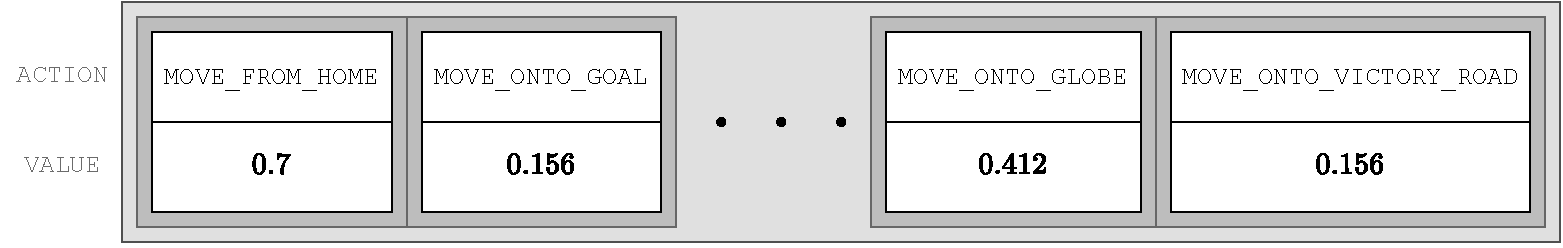
\includegraphics[width=\textwidth]{fig/genome_rep_list.drawio.pdf}
		\end{center}
		\caption{Example of chromosome representation for GA.}
		\label{fig:chromosome_rep}
\end{figure}
The chromosome representation of each player individual is a list of genes in the form of couples, where the 
first element is the enum corresponding to a possible action e.g. \texttt{MOVE\_FROM\_HOME}
while the second element is the value associated with the action. Here actions of greater value
are associated with greater importance. This chromosome representation can be seen exemplified in figure~\ref{fig:chromosome_rep}.
This representation is used due to it containing a great variety of possible actions
during a game, while being compact enough to not contain all possible states.
The standard floating point mutation is performed by having a 5\% probability of
adding a value $\delta\in[-1,1]$ chosen uniformly in the interval.
The goal is thus to determine which actions are better than others, by changing their values such
that the action with the greatest value in a state, generally causes the individual to win more often.
Thus the end result being a ranked list of all actions, from least important action to the most.\par
\begin{table}
	\begin{center}
		\caption{Actions available to the player}
		\label{tab:actions}
		\begin{tabular}[c]{|l|}
			\hline
			Actions \\ \hline
			\texttt{MOVE\_FROM\_HOME} \\
			\texttt{MOVE\_FROM\_HOME\_AND\_KILL} \\
			\texttt{MOVE} \\
			\texttt{MOVE\_ONTO\_STAR} \\
			\texttt{MOVE\_ONTO\_STAR\_AND\_DIE} \\
			\texttt{MOVE\_ONTO\_STAR\_AND\_KILL} \\
			\texttt{MOVE\_ONTO\_GLOBE} \\
			\texttt{MOVE\_ONTO\_GLOBE\_AND\_DIE} \\
			\texttt{MOVE\_ONTO\_ANOTHER\_DIE} \\
			\texttt{MOVE\_ONTO\_ANOTHER\_KILL} \\
			\texttt{MOVE\_ONTO\_VICTORY\_ROAD} \\
			\texttt{MOVE\_ONTO\_GOAL} \\
			\hline
		\end{tabular}
	\end{center}
\end{table} 
In order to include the current state into the decision making, the actions which are impossible
are filtered away when playing the game, such that the agent only is offered the legal actions 
for this particular state. Which ever action has the highest value is then chosen, 
and the game continues.
The different possible actions can be seen in table~\ref{tab:actions}.
One example of such a chromosome can be seen in table~\ref{tab:action-value-paris-example}
with the actions ranked in table~\ref{tab:ranked-action-value-pair-example}. \par
\begin{table}[!htb]
    \begin{minipage}[b]{.5\linewidth}
		\centering
		\caption{Action value pairs example}
		\label{tab:action-value-paris-example}
        \begin{tabular}{|l|l|} \hline
			Action & Value \\ \hline
			\texttt{MOVE\_FROM\_HOME} & 0.785\\
			\texttt{MOVE\_FROM\_HOME\_AND\_KILL} & 0.288\\
			\texttt{MOVE} & 0.512\\
			\texttt{MOVE\_ONTO\_STAR} & 0.339\\
			\texttt{MOVE\_ONTO\_STAR\_AND\_DIE} & 0.023\\
			\texttt{MOVE\_ONTO\_STAR\_AND\_KILL} & 0.591\\
			\texttt{MOVE\_ONTO\_GLOBE} & 0.973\\
			\texttt{MOVE\_ONTO\_GLOBE\_AND\_DIE} & 0.448\\
			\texttt{MOVE\_ONTO\_ANOTHER\_DIE} & 0.915\\
			\texttt{MOVE\_ONTO\_ANOTHER\_KILL} & 0.284\\
			\texttt{MOVE\_ONTO\_VICTORY\_ROAD} & 0.488\\
			\texttt{MOVE\_ONTO\_GOAL} & 0.672\\	\hline
        \end{tabular}
    \end{minipage}%
	\begin{minipage}[b]{.5\linewidth}
      \centering
	  \caption{Ranked action value pairs example}
	  \label{tab:ranked-action-value-pair-example}
	  	\begin{tabular}{|l|l|l|}\hline
			Ranking & Action & Value \\ \hline
			1& \texttt{MOVE\_ONTO\_STAR\_AND\_DIE}  & 0.023\\
			2& \texttt{MOVE\_ONTO\_ANOTHER\_KILL}   & 0.284\\
			3& \texttt{MOVE\_FROM\_HOME\_AND\_KILL} & 0.288\\
			4& \texttt{MOVE\_ONTO\_STAR}            & 0.339\\
			5& \texttt{MOVE\_ONTO\_GLOBE\_AND\_DIE} & 0.448\\
			6& \texttt{MOVE\_ONTO\_VICTORY\_ROAD}   & 0.488\\
			7& \texttt{MOVE}                        & 0.512\\
			8& \texttt{MOVE\_ONTO\_STAR\_AND\_KILL} & 0.591\\
			9& \texttt{MOVE\_ONTO\_GOAL}            & 0.672\\
			10& \texttt{MOVE\_FROM\_HOME}            & 0.785\\
			11& \texttt{MOVE\_ONTO\_ANOTHER\_DIE}    & 0.915\\
			12& \texttt{MOVE\_ONTO\_GLOBE}           & 0.973\\ \hline
		\end{tabular}
	\end{minipage} 
\end{table}
To determine when the algorithm has converged, generally the lack of variation between generations' 
performance can be used, however due to the great variance introduced in Ludo through the dice roll, 
an alternative must be applied. Here a configuration with a crossover rate of $50\%$ and tournament 
selection was made to run until it appeared reasonable to conclude that the algorithm had converged.
The metric chosen to represent a generations performance is the average of all individuals' average
win rates. The number of games played to determine an average win rate for one individual is chosen to be $50$.\par
By inspection the number of generations necessary for convergence was found to be approximately $150$
generations as seen in figure~\ref{fig:convergence}.
\begin{figure}[h]
	\begin{center}
		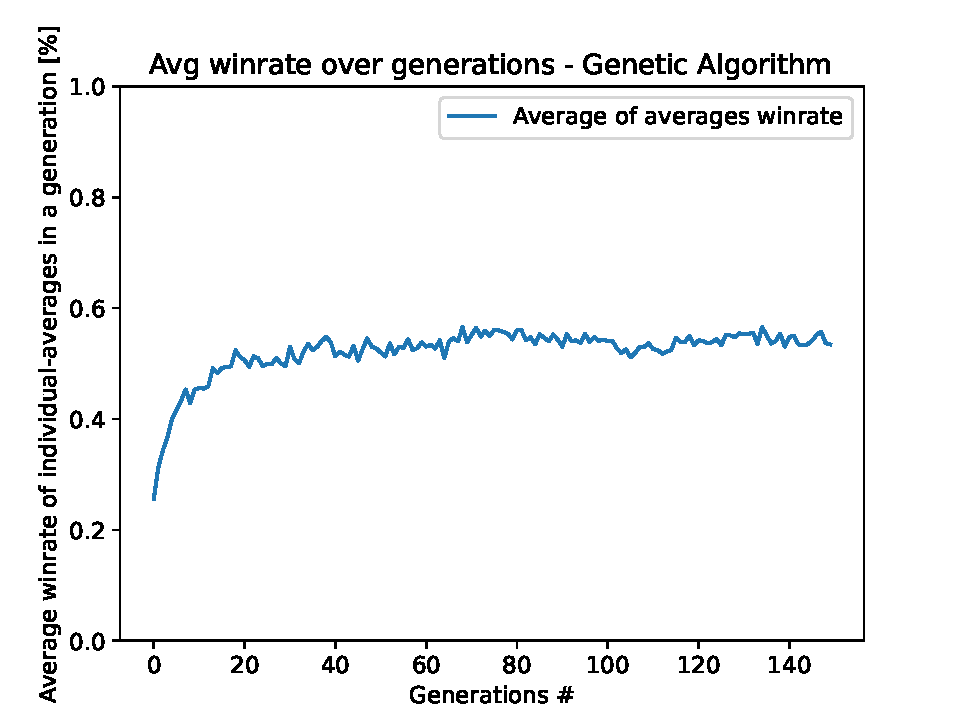
\includegraphics[width=0.7\textwidth]{fig/img_cr_0.5_se_tournament.pdf}
	\end{center}
	\caption{Convergence of GA with a crossover rate of $50\%$ and tournament selection}
	\label{fig:convergence}
\end{figure}
When starting the algorithm $100$ individuals are generated, each with random action values between $0$ and $1$.\par
Each individual is then set to play the before mentioned $50$ games against three dummy players who make 
random moves among the legal
ones presented. By choosing the dummies to be random, an increase in average win rate will indicate 
improvements beyond random variation. \par 
After each individual has played their $50$ games, a fitness score is calculated based on their performance using 
the fitness function in equation (\ref{eq:fitness})
\begin{equation}
	S_{fit} = \overline{WR} \cdot \left( \overline{N}_{kill} + \overline{N}_{tog} \right)
	\label{eq:fitness}
\end{equation}
In this expression $S_{fit} \in \mathbb{R}$ is the fitness score for some particular individual,
$\overline{WR} \in \mathbb{R}$ is the average win rate for said individual after its $50$ games played,
$\overline{N}_{kill}\in\mathbb{R}$ is the number of enemy tokens the player has sent home and
$\overline{N}_{tog} \in \mathbb{R}$ is the average number of tokens the player got to place 
on the goal. \par
This fitness function is formulated such that the win rate scales the other attributes,
making it the dominant trait. The other attributes such as number of tokens on the goal is 
used to encourage a more aggressive play style, while compensated for by the defensive play 
style of killing opponents tokens when possible. By using the win rate as a scaling factor,
an individual with 0 wins will never get to reproduce minimizing the opportunity for undesired fitness exploits. \par
Given (\ref{eq:fitness}), the 6 configurations presented in table~\ref{tab:configs} are
run with the parameters described above. The results can be seen in 
figure~\ref{fig:configs_tested}.
\begin{figure}[h]
	\begin{center}
		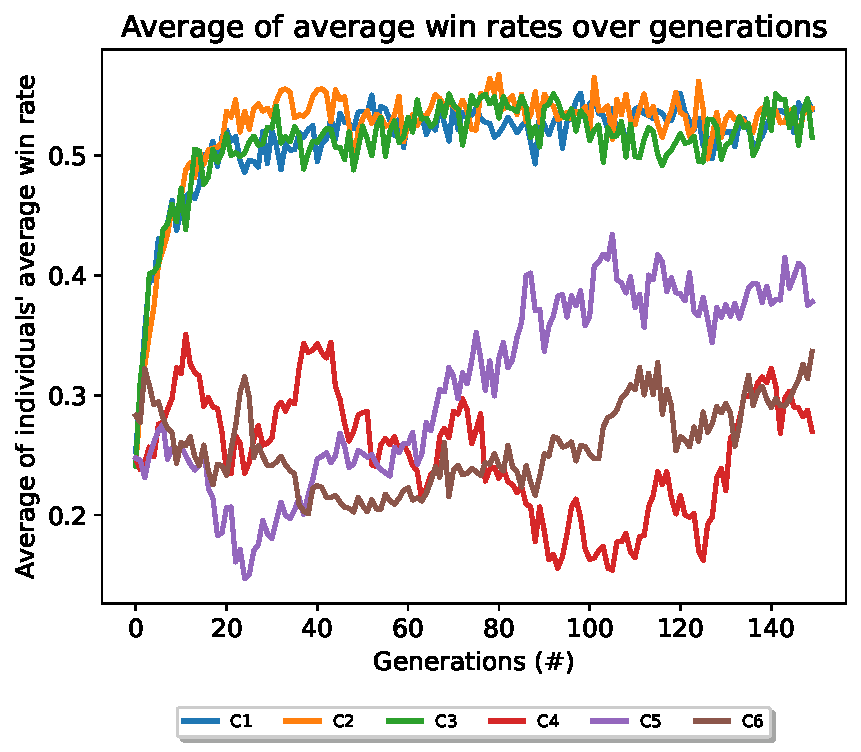
\includegraphics[width=0.7\textwidth]{fig/config_plot.pdf}
	\end{center}
	\caption{Performance of configurations presented in table~\ref{tab:configs}}
	\label{fig:configs_tested}
\end{figure}
Here each data point is the average of average win rates from each 
generation.\par 
To determine if any of the 6 configurations perform statistically best, the 
chromosome with the greatest average win rate from each configuration over all generations are chosen 
as representatives for said configuration. \par
Each of these is set to play $50$ games $1000$ times. These $1000$ win rates are then used to
checked for normality with a Shapiro-Wilk's test, then for equal variance with either a Bartlett
test or a Levene's test depending on the outcome of the previous. A type of ANOVA is then applied
to determine if any of the variables are cause a statistically significant difference. 
This type of ANOVA is dependent on the results from the previous tests.
Finally a 2 sample t-test is applied to determine the best configuration.

\subsection{Comparison of Algorithms}

The best chromosome produced by the algorithm described above will be compared to the 
best chromosome produced in paper \cite*{peter}. The best algorithm produced by this paper 
uses a population size of 128, a cross over rate of 75\%, the bits per crossover is 10\%, 
variant uniform crossover, standard binary mutation, a mutation rate of 1\%, a binary chromosome 
representation and 10\% elitism.

% The algorithm used as comparison to the algorithm of this paper as described above,
% uses a GA algorithm with chromosome representation identical to the one presented 
% in this paper, except the genes are binary. 



% The metric used to determine the performance of any generation, each individual determine its average win rate over 
% the $50$ games played, and each of these averages are applied in a average of averages over the generation.
% By inspection the number of generations necessary for convergence was found to be approximately $150$
% generations as seen in figure~\ref{fig:convergence}. 
% Using this as the baseline for comparison, each configuration in table~\ref{tab:configs} can be compared. \par


	% You do need to describe your representation of the problem and how you encoded it
	% (and why you chose that representation); 

	% you should describe any non-standard choices
	% for operators or procedures; you should state what choices you made for the parameters
	% (e.g. learning rate) and how you chose them (e.g. preliminary test, found in a paper
	% (cited), guessed, etc.); you should describe the tests you conducted to ensure your code
	% works as you claim. Describe what experiments you did.

% You are expected to describe one AI method quite completely (your “own”
% one) and a second one much more briefly. The second one is the one you will be
% comparing against and will have been implemented, and described in detail, by someone
% else (e.g. a partner in your group). Remember to cite and/or acknowledge the source for
% this second method.
% The two methods can be different algorithms, e.g. GA vs. Q-learning, or they can be
% two instances of the same algorithm using different game representations. You are free
% to compare more methods or to try to isolate important factors if you wish, but do not
% exceed the page limit of the paper format.


\section{Results}
\label{sec:Results}
Given the win rates from section~\ref{sec:Methods}
a Shapiro-Wilk's test is applied to each configuration
resulting in the p-values shown in table~\ref{tab:shapiro-wilks}
\begin{table}[H]
	\begin{center}
		\caption{P-values from applying Shapiro-Wilk's test on win rates over $1000$ games}
		\label{tab:shapiro-wilks}
		\begin{tabular}[c]{|c|l|}
			\hline
			Configuration &     p-value             \\ \hline
			C1            &    $1.53\cdot10^{-5}$   \\
			C2            &    $8.01\cdot 10^{-6}$  \\
			C3            &    $4.33\cdot 10^{-5}$  \\
			C4            &    $3.08 \cdot 10^{-5}$ \\ 
			C5            &    $7.47\cdot 10^{-6}$  \\ 
			C6            &    $3.36\cdot10^{-6}$   \\ \hline
		\end{tabular}
	\end{center}
\end{table}
Due to all the p-values presented in table~\ref{tab:shapiro-wilks}
being less than $0.05$, its concluded that all win rate samples
are not normally distributed.
However due to Shapiro-Wilk's test being a non-parametric method designed to test for 
theoretical normality i.e. the perfect bell curve, in large samples these tests are overpowered 
to detect minor deviations from normality, thus false negatives for normality are likely produced.
For this reason a qq-plot is applied to determine the configurations normality. 
The result can be seen in figure~\ref{fig:qqplots}.
\begin{figure}[h]
	\begin{small}
		\begin{center}
			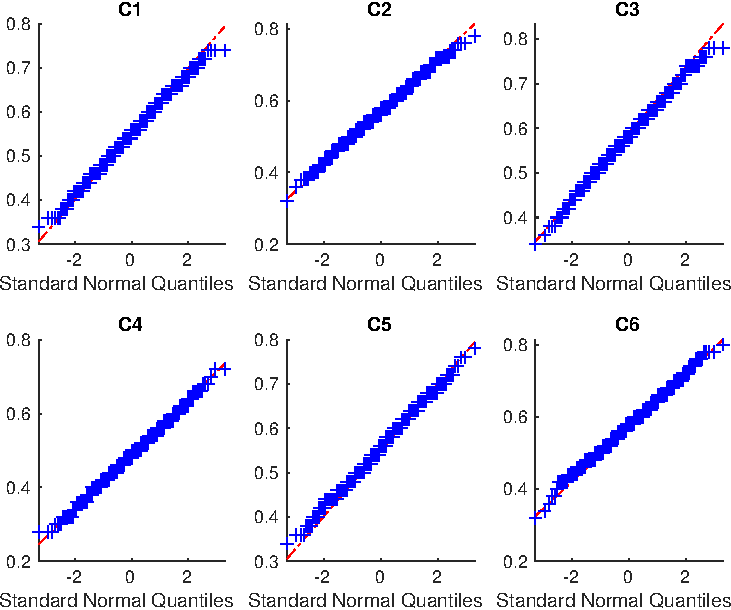
\includegraphics[width=0.7\textwidth]{fig/myfigure.pdf}
		\end{center}
		\caption{qq-plots showing the normality for avg win rates of each configuration}
		\label{fig:qqplots}
	\end{small}
\end{figure}
Based on these results it is concluded that all the average win rates are in fact normally
distributed.
To determine if all the samples have equal variance the Bartlett test was applied which resulted in a 
p-value of approximately $0.897$. Since this value is greater than $0.05$, it is concluded that
 all the avg win rate samples have equal variance.
Finally to test if the configurations perform statistically 
significantly different, a two factor ANOVA is applied 
due to the previous statistical findings. 
The result of this test can be seen in table~\ref{tab:2-factor-anova-table}
\begin{table}[H]
	\begin{center}
		\caption{ANOVA table from an two factor ANOVA test between the crossover rate and selection methods effect on avg win rate}
		\label{tab:2-factor-anova-table}
		\begin{tabular}{|l|l|l|l|l|}
			\hline
			{} &     sum sq &      df &           F &         p-value \\ \hline
			crossover rate                     &   3.98 &     2.00 &  398.68 &   $2.75\cdot 10 ^{-163}$ \\
			selection method                   &   1.15 &     1.00 &  231.70 &   $2.28\cdot 10^{-51}$   \\
			crossover rate:selection method    &   0.95 &     2.00 &   95.80 &   $1.10\cdot 10^{-41}$   \\
			Residual                           &  29.98 &  5994.00 &         &                          \\ \hline
		\end{tabular}
	\end{center}
\end{table}
As it here can be seen the p-values for each tested case rejects the null hypothesis, meaning the 
samples does not come from the same distribution. To determine which configuration performs the best,
each configuration's samples mean is found as shown in table~\ref{tab:mean-and-variance}.
It can here be seen that the best configuration is C3 with a mean avg win rate of $58.3\%$. 
Here a repeated 2 sample t-test is applied between C3 and the other configurations
to determine if there is statistical evidence to support that any of the other configurations 
are from the same distribution, resulting in the p-values presented in table~\ref{tab:2-sample-t-test}.
\begin{table}[!htb]
    \begin{minipage}{.5\linewidth}
		\centering
		\caption{Mean for all configurations C1-C6}
		\label{tab:mean-and-variance}
        \begin{tabular}{|l|l|} \hline
					Conf.         &  Mean  \\ \hline
					C1            &  0.550 \\
					C2            &  0.569 \\
					C3            &  0.583 \\
					C4            &  0.487 \\
					C5            &  0.556 \\
					C6            &  0.577 \\\hline
        \end{tabular}
    \end{minipage}%
	\hspace{0.3cm}
	\begin{minipage}{.5\linewidth}
      \centering
	  \caption{2 sample t-test between C3 \\ and other configurations}
	  \label{tab:2-sample-t-test}
	  	\begin{tabular}{|l|l|l|}\hline
				  Conf. comparison & p-values    \\ \hline
				  C3/C1 & $5.617\cdot 10^{-25 }$ \\
				  C3/C2 & $1.631\cdot 10^{-05 }$ \\
				  C3/C4 & $5.226\cdot 10^{-165}$ \\
				  C3/C5 & $1.025\cdot 10^{-17 }$ \\
				  C3/C6 & 0.044 \\ \hline
		\end{tabular}
	\end{minipage} 
\end{table}
As it here can be seen no other configuration comparison results in a p-value greater than
$0.05$, with C6 being the closest at $0.044$, and thus C3 is the best found configuration.\par



\section{Analysis and Discussion}
\label{sec:Analysis and Discussion}
In order to compare this paper's best configuration's performance with the one found in 
paper \cite{peter},
each best configuration is set to play 50 games 1000 times. 
Since this paper's best configuration already 
is found to be normally distributed in its average win rate, the comparative paper's best 
configuration is tested resulting in the qq-plot shown in figure~\ref{fig:peter-qq-plot}.
\begin{figure}
	\begin{small}
		\begin{center}
			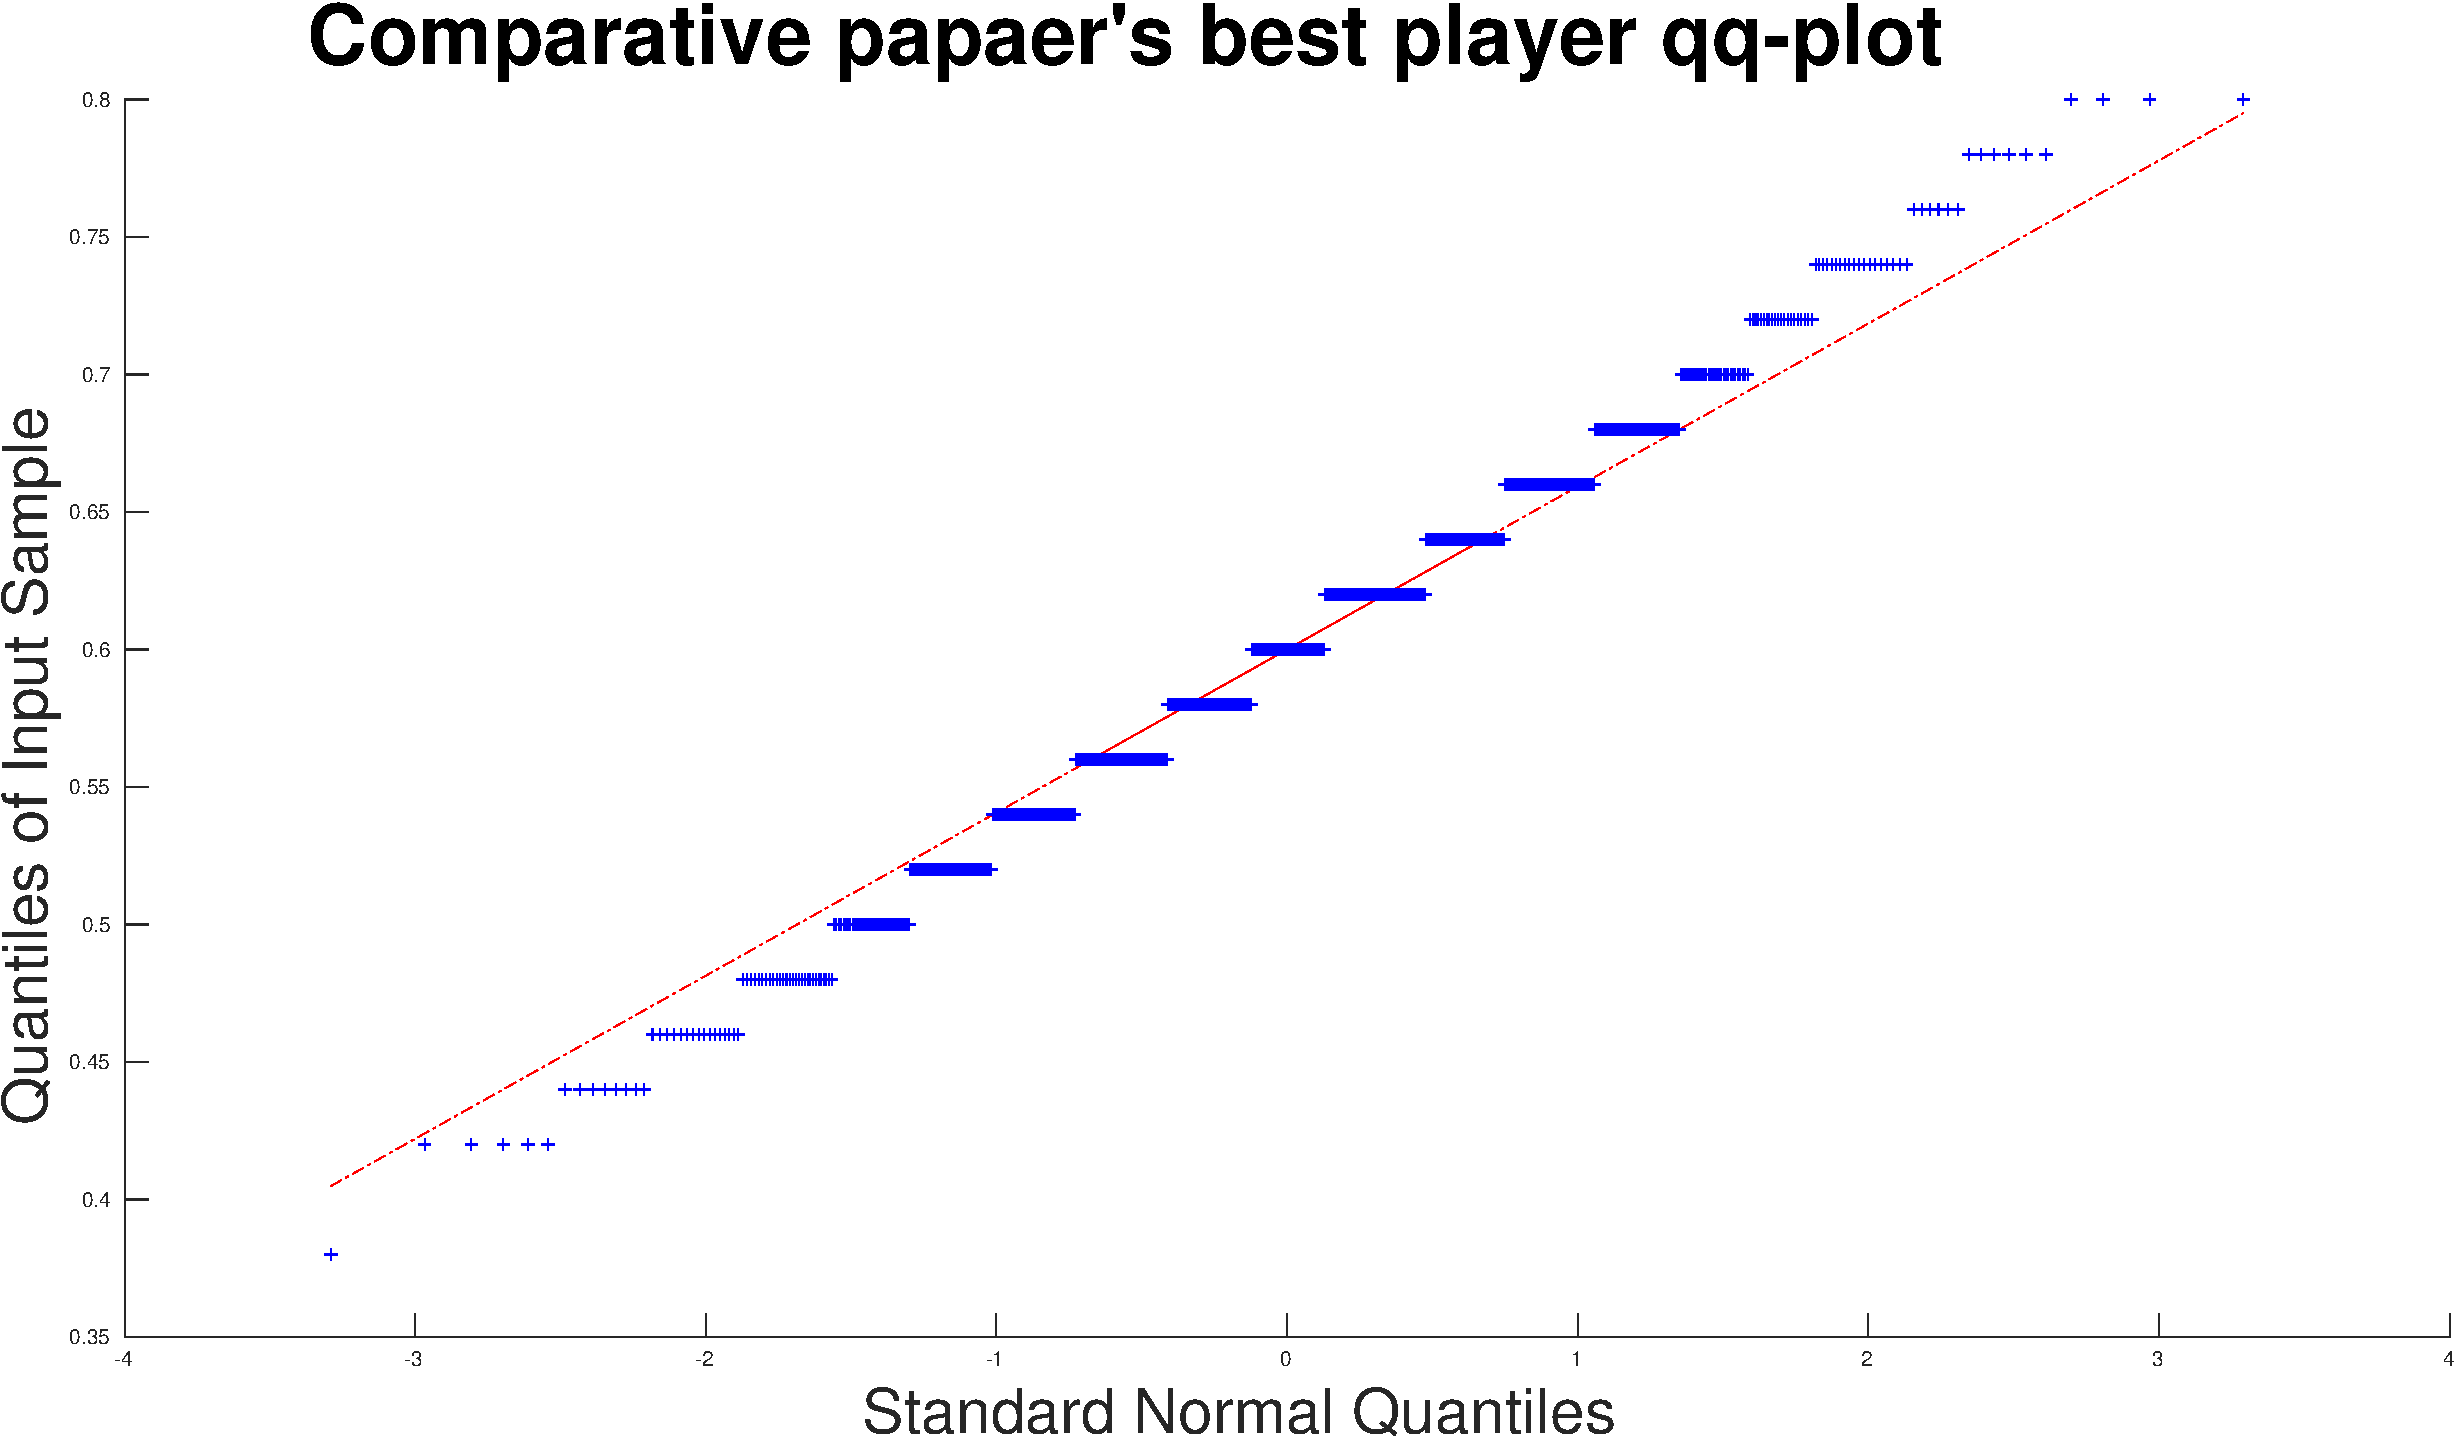
\includegraphics[width=0.9\textwidth]{fig/peter-qq-plot.pdf}
		\end{center}
		\caption{qq-plot of the comparative paper's best configuration win rate over 50 games 1000 times}
		\label{fig:peter-qq-plot}
	\end{small}
\end{figure}
Based on the found qq-plot it is concluded that the comparative paper's configuration 
data are sufficiently normality distributed. A Bartlett test is then performed to test for equal variance. 
Here a p-value of $0.52$ is found, and thus it is assumed that the samples have equal variance. 
All the necessary criteria has now been fulfilled to perform a 2 sample t-test to assert
if there is statistical evidence to support that the two configurations are from different underlying 
normal distributions.
Here a p-value of approximately $ 2.9\cdot 10^{-17}$ is found, 
and thus the samples are not of the same distribution. Finally to determine which configuration 
performs the best, the mean is found for each algorithm as shown in table~\ref{tab:final-result}
\begin{table}[H]
	\begin{center}
		\caption{Means of C3 and the best configuration from the comparative paper}
		\label{tab:final-result}
		\begin{tabular}{|l|l|}
			\hline
			{}					& Mean   \\ \hline
			C3					& 0.583  \\ \hline
			Comparative paper 	& 0.609 \\ \hline
		\end{tabular}
	\end{center}
\end{table}
It can here be seen that the best configuration is produced by the comparative paper
with a mean avg win rate of $60.9\%$ compared to the one found in this paper at $58.3\%$.
The ranked lists of the two best configurations can be seen in table~\ref{tab:ranked-victor}
for this paper, and for the comparative paper in table~\ref{tab:ranked-peter}
\begin{table}[!htb]
    \begin{minipage}[b]{.5\linewidth}
		\centering
		\caption{The ranked actions from the chromosome of C3 from this paper}
		\label{tab:ranked-victor}
        \begin{tabular}[t]{|l|l|l|} \hline
			Ranking & Action & Value \\ \hline
			0  & \texttt{            MOVE\_FROM\_HOME }&  3.451 \\
			1  & \texttt{    MOVE\_ONTO\_ANOTHER\_DIE }&  1.098 \\
			2  & \texttt{                        MOVE }&  0.912 \\
			3  & \texttt{ MOVE\_ONTO\_GLOBE\_AND\_DIE }&  0.791 \\
			4  & \texttt{   MOVE\_ONTO\_VICTORY\_ROAD }&  0.789 \\
			5  & \texttt{ MOVE\_ONTO\_STAR\_AND\_KILL }&  0.394 \\
			6  & \texttt{            MOVE\_ONTO\_GOAL }&  0.193 \\
			7  & \texttt{           MOVE\_ONTO\_GLOBE }& -0.198 \\
			8  & \texttt{            MOVE\_ONTO\_STAR }& -0.389 \\
			9  & \texttt{ MOVE\_FROM\_HOME\_AND\_KILL }& -0.596 \\
			10 & \texttt{  MOVE\_ONTO\_STAR\_AND\_DIE }& -2.303 \\
			11 & \texttt{   MOVE\_ONTO\_ANOTHER\_KILL }& -5.480 \\ \hline
        \end{tabular}
    \end{minipage}%
	\hspace{0.3cm}
	\begin{minipage}[b]{.5\linewidth}
      \centering
	  \caption{The ranked actions from the chromosome of the best configuration from the comparative paper}
	  \label{tab:ranked-peter}
	  	\begin{tabular}[t]{|l|l|l|}\hline
			Ranking & Action & Value \\ 
			\hline
			0  & \texttt{MOVE\_FROM\_HOME\_AND\_KILL}&   237 \\
			1  & \texttt{MOVE\_ONTO\_GOAL}&              235 \\
			2  & \texttt{MOVE\_ONTO\_ANOTHER\_KILL}&     228 \\
			3  & \texttt{MOVE\_ONTO\_STAR\_AND\_DIE}&    181 \\
			4  & \texttt{MOVE\_ONTO\_STAR\_AND\_KILL}&   119 \\
			5  & \texttt{MOVE\_FROM\_HOME}&              97 \\
			6  & \texttt{MOVE\_ONTO\_STAR}&              95 \\
			7  & \texttt{MOVE\_ONTO\_VICTORY\_ROAD}&     93 \\
			8  & \texttt{MOVE\_ONTO\_GLOBE}&             86 \\
			9 & \texttt{MOVE}&                          83 \\
			10 & \texttt{MOVE\_ONTO\_ANOTHER\_DIE}&      65 \\
			11 & \texttt{MOVE\_ONTO\_GLOBE\_AND\_DIE}&   16 \\ 
			\hline
		\end{tabular}
	\end{minipage} 
\end{table}

When considering the shown difference in performance, the hyper parameters of interest 
include the generation size, the lower mutation rate, the selection method,
the chromosome representation and the use of elitism.\par
The generation size being 128 compared to the one used in this paper of 100, 
explains part of the difference in performance, since a wider search provides more 
opportunities for well performing solutions.
For a lower introduction of new genetic material, the comparative paper applies a
lower mutation rate of 1\%, which is less likely destroy useful genes.
Combined with the use of elitism, a greater emphasis is placed on conserving 
well performing genetic material.
The comparative paper uses a roulette selection method, which in this paper was demonstrated to 
provide inferior results compared to tournament selection. 
The possible downsides of roulette selection are likely 
mitigated by greater genetic preservation in the comparative paper. 
Another possibility could be that roulette selection does provide greater 
benefits with the comparative paper's other configurations, though based on 
the great similarity between the algorithms, this seems unlikely.\\
Possible improvements to the methods in this paper include 
a greater number of games to represent individual's performance and 
a more detailed action space representation.
Here 100 games would be a beneficial improvement from the 50 games used, 
and a more detailed action space representation \\ (e.g. \texttt{MOVE\_INTO\_DANGER})
would give more nuanced representation of the games current state.
However this would add significant computational complexity to the method, 
resulting in a large time penalty and require more computational 
resources than available for this project.
Finally while the mean avg win rates of the two configurations are 
relatively close, the actions rankings have very little overlap. How exactly
said overlap result in such similar avg win rates require further research.


\section{Conclusion}
\label{sec:Conclusion}

To conclude this paper has applied 6 different configurations of GA to the game Ludo
and found configuration C3 to have the best performance with a mean avg win rate of 58.3\%.
This configuration was then compared to the best 
from a comparative paper\cite*{peter} which used a different set of hyperparameter configurations
and chromosome representation with a mean avg win rate of 60.9\%. The comparison showed that 
the GA from the comparative paper performs statically significantly better than the 
one found in this paper. The difference between the configurations was then discussed 
with possible changes and improvements to the approach applied in this paper.


\section{Acknowledgements}
\label{sec:Acknowledgements}

I thank Peter Ørholm Nielsen for providing the work behind the comparative 
paper~\cite*{peter}, enabling the work done and conclusions derived during this work.
 


\printbibliography %Prints bibliography



\end{document}